\section{Ejercicio 3}
\subsection*{Instrucción}
Cuando los clientes de la empresa de alquiler de coches alquilan un coche, el sistema que estamos construyendo
tiene que proporcionarles el precio del alquiler. Este precio lo calcula la operación \texttt{getPrice() : Integer} de la siguiente
forma: El precio base será el precio del modelo del vehículo por día.
\begin{center}
    \texttt{ (pricePerDay) * [endDate - startDate]}
\end{center}
Además, la empresa de alquiler de coches puede añadir al cálculo de precios la posibilidad de hacer promociones
que implican descuentos de estos precios. Inicialmente, la empresa ofrecerá dos tipos de promociones: por cantidad
y por porcentaje.
\begin{itemize}
    \item \textbf{Promoción por cantidad:} permitirá decrementar el precio del alquiler en la cantidad indicada en
    la promoción.
    \item \textbf{Promoción por porcentaje:} decrementará el precio del alquiler en el porcentaje indicado en la
    promoción. Las promociones se asignan a los alquileres en el momento de su creación.
\end{itemize}
Evidentemente, es posible
que a algunos alquileres no se les aplique ninguna promoción. Las promociones que se asignan a los alquileres son
determinadas por una política de la empresa que no impacta al diseño de nuestra operación (impactará a la
operación que crea los alquileres).\par
\vspace{0.15cm}
Eso sí, la empresa quiere que mientras no se haga el pago del alquiler, si aparecen
nuevas promociones, se apliquen a los alquileres siempre y cuando sean más favorables (no nos tenemos que
preocupar tampoco de estos cambios, son gestionados por otras operaciones).


\subsection{Patrón de Diseño utilizado}
Para poder realizar este apartado optamos varias casuisticas de diferentes patrones de diseño validos. Por un lado optamos por el patron visitante,
dicho patron complicaria demasiado la imlementación de la operacion debido al gran numero de instancias presentes de dicho patron para un unico metodo,esto hace que 
el uso de este patron sea algo ineficiente. Tras ese planteamiento llegamos a la conclusion de utilizar el patron \textbf{Strategy} para poder implementar la operacion correctamente.
Este patron se basa en la utilizacion de una interfaz que actua como padre de todos los objetos que implementen una operacion similar, en este caso tenemos dos tipos de promociones,
\textbf{Promoción por porcentaje} y \textbf{Promoción por cantidad} ambas mantienen una logica similar por lo que el uso del patron \textbf{Strategy} es el adecuado.

\subsection{Efectos sobre el Diagrama de Diseño}

\begin{figure}[H]
    \centering
     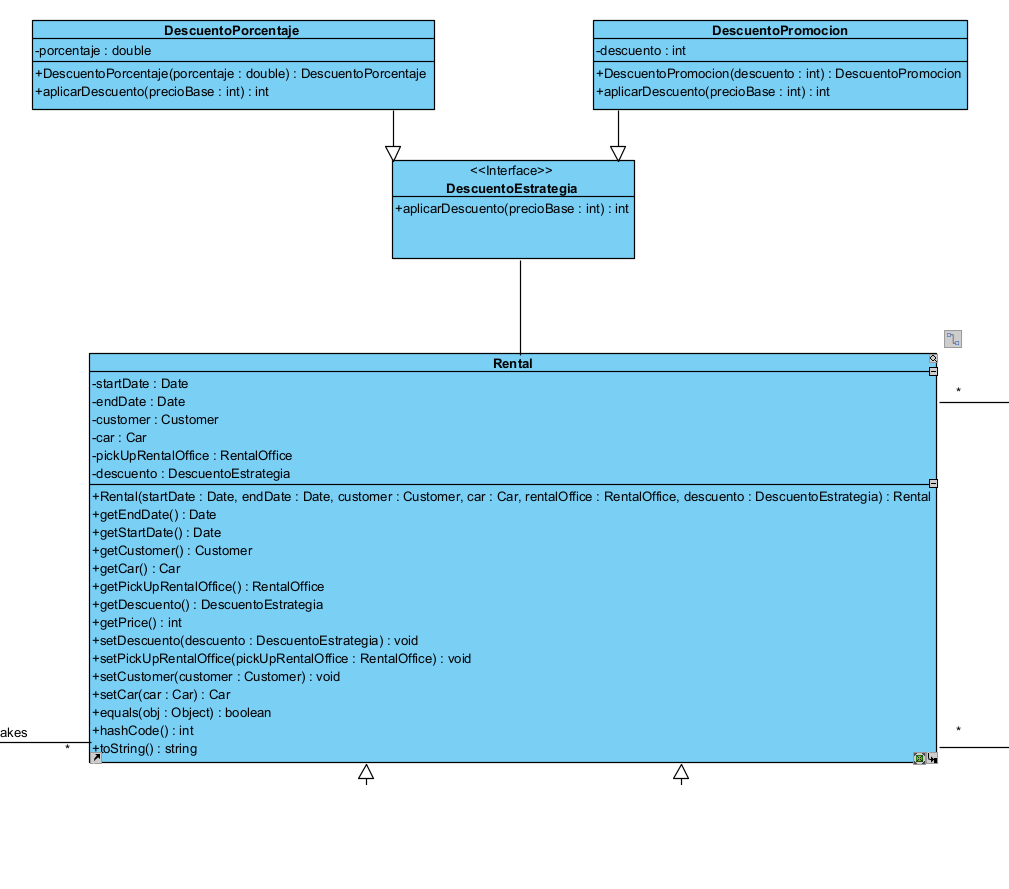
\includegraphics[width=1\linewidth]{assets/diagramas/UML_Apartado3.png}
     \caption{Diagrama de Diseño del apartado 3}
\end{figure}

Como podemos observar, el patron \textbf{Strategy} mantiene una interfaz padre de la cual heredan todas las instancias de objetos que vayan a realizar dicha operacion.
Como bien hemos dicho antes nos basamos en un sistema con dos operaciones diferentes para obtener el precio final, por lo cual necesitaremos crear dos clases una para cada tipo de 
promocion. Estas heredaran de la clase \textbf{Strategy} para asi obligar al sistema a implementar dichas operaciones en cada una de las clases. Un requisito del sistema es que dichas
promociones se apliquen al instanciar un objeto \textbf{Rental}, es por eso que dichos tipos de promociones vendran instanciados en el constructor de dicha clase pudiendo ser nulo en caso 
de que no se le aplique ningun tipo de promocion.\par

\subsection{Implementación de \textit{getPrice() : Integer}}
\begin{lstlisting}[style = javaNormal, language=Java] 

    introducir codigo aqui

\end{lstlisting}\par
En la primera seccion podemos encontrar las nuevas instancias que debemos generar para poder usar el patron \textbf{Strategy} dichas clases implementan el metodo de la interfaz
de manera similar pero cambiando ligeramente la forma en la que calculan los precios a dependiendo de sus propios parametros privados (porcentaje o cantidad).\par
\vspace{0.15cm}
Para implementar el metodo getPrice hemos decidido generar a partir de los parametro \textbf{startDate} y \textbf{endDate} el precio base que tendria el alquiler antes de aplicar 
cualquier tipo de promocion. Como bien hemos explicado antes en caso de que no exista promocion alguna se instanciara como nulo el atributo en el constructor. Es por eso que 
antes de calcular el nuevo precio comprobamos si el \textbf{Rental} contiene un tipo de promocion disponible, en caso contrario devolveremos el precio base inicial.
\newpage
